\documentclass[10pt,journal,compsoc]{IEEEtran}

\usepackage[T1]{fontenc}
\usepackage{graphicx}
\usepackage{booktabs}
\usepackage{array}
\usepackage{tabularx}
\usepackage{amsmath,amssymb}
\usepackage{microtype}
\usepackage{url}
\usepackage[hidelinks]{hyperref}
\setcounter{dbltopnumber}{2}
\renewcommand{\dbltopfraction}{0.95}
\renewcommand{\textfraction}{0.05}

\newcommand{\system}{KubeML-Aware}
\newcommand{\jct}{\mathrm{JCT}}

\begin{document}

\title{KubeML-Aware: Kubernetes-Native Rank-Aware Admission for Burst-Submitted ML Training}

\author{Amir Mirzaei Movahed and Majid Bafandeh%
\IEEEcompsocitemizethanks{%
\IEEEcompsocthanksitem Amir Mirzaei Movahed: \href{mailto:Amir.m.movahed@ut.ac.ir}{Amir.m.movahed@ut.ac.ir}.
\IEEEcompsocthanksitem Majid Bafandeh: \href{mailto:majidb@aut.ac.ir}{majidb@aut.ac.ir}.}}

\markboth{Manuscript prepared for journal review, 2026}{Mirzaei Movahed and Bafandeh: KubeML-Aware}
\maketitle

\begin{abstract}
Kubernetes makes mature placement decisions for Pods, but its default policy does not infer the relative value of machine-learning (ML) training jobs from their convergence and workload characteristics. This distinction matters when heterogeneous jobs arrive as a burst and compete on the same node. We present \system, a training-specific admission layer that leaves feasibility checks, node scoring, and binding to the default scheduler. The system collects a complete burst, derives a deterministic rank from six annotated characteristics, and controls scheduling eligibility through stable Pod scheduling gates. A fail-closed FastPath uses bounded CPU demand and fresh node telemetry to prefill the scheduler queue when progress can be established; a small tail optimizer may rearrange only the lowest-ranked jobs. We implemented the controller as an in-cluster service and evaluated the deployed path by executing real Kubernetes Jobs on a shared four-core K3s node. The controlled NumPy trainer performs matrix operations, gradient-buffer updates, synchronization copies, and checkpoint I/O. Five paired repetitions compared 12 heavy jobs under synchronized FIFO admission and \system. Mean job completion time fell from 31.047 to 28.755~s, a mean paired improvement of 7.31\% (exploratory 95\% CI [2.57\%, 12.05\%]). Makespan moved in the same direction (55.369 to 54.005~s, 2.47\%) and decreased in all five pairs, but its paired interval includes zero, so we report it as directional rather than an established effect. These measurements support the feasibility of Kubernetes-native, rank-aware admission, but they are a small CPU-only pilot on a non-isolated node; they do not establish general performance for GPU or multi-node training.
\end{abstract}

\begin{IEEEkeywords}
Kubernetes, machine-learning training, scheduling gates, admission control, job ranking, job completion time.
\end{IEEEkeywords}

\section{Introduction}

Training workloads rarely behave as interchangeable batch jobs. Even when two Pods request the same CPU and memory, their useful work can differ in duration, convergence rate, matrix or tensor scale, synchronization volume, and checkpoint frequency. Production traces show that this heterogeneity is a central difficulty in ML cluster management, alongside queueing delay and uneven accelerator utilization~\cite{weng2022mlaas}. When a set of jobs is submitted together, the admission order can therefore change which jobs obtain early access to a contested node and how quickly the burst clears.

Kubernetes exposes a rich scheduling framework for deciding \emph{where} a Pod may run. The default scheduler filters infeasible nodes, scores the remaining candidates, and binds each Pod while respecting requests, taints, affinity, storage, and topology constraints~\cite{kubernetesSchedulingFramework}. It does not, however, derive a burst-relative priority from training behavior. A PriorityClass can express importance chosen by an operator, but it does not estimate that importance from ML features. Replacing the scheduler is one way to add such a policy, although it also creates the burden of reproducing or safely composing with mature placement logic.

This paper studies a narrower alternative: change when a training Pod becomes eligible for the existing scheduler, without replacing node selection. \system{} uses Pod Scheduling Readiness~\cite{kubernetesSchedulingReadiness} to hold every member of an annotated burst behind a scheduling gate. Once the complete burst is present, a controller validates six features, calculates a deterministic order, and removes the gates according to a resource-aware policy. Gate removal does not bind a Pod or reserve a node; the default scheduler remains the placement authority.

The ranking model originates from the six-feature formulation in~\cite{abdelshaheed2025intelligent}, but the deployed system differs materially from a manual-binding reproduction. It adds complete-burst validation, stable scheduling gates, resource-bounded manifests, fresh Metrics API feedback, crash-safe records, structured application-level start evidence, and a FastPath that avoids controller-induced gaps. The evaluation reports only measurements generated by this implementation. Published percentages from the source formulation are not treated as results of \system{} or as a head-to-head comparison because the two studies used different implementations, workloads, and environments.

The paper makes three contributions:
\begin{itemize}
  \item a deterministic, burst-relative training rank with explicit validation, normalization, and tie handling;
  \item a Kubernetes-native controller that applies the rank through scheduling gates and a fail-closed, telemetry-aware FastPath while retaining \texttt{default-scheduler}; and
  \item a paired real-cluster pilot that executes identical physical CPU workloads in both arms and measures mean JCT and burst makespan from application-emitted events.
\end{itemize}

The evidence is deliberately bounded. The workload is a controlled training proxy rather than a neural-network benchmark; the cluster has one shared CPU node; and the five repetitions are insufficient for broad claims about other workloads or environments. The aim is to establish an auditable production path and a credible first measurement, not to claim an optimal general-purpose ML scheduler.

\section{Background and Related Work}

\subsection{Kubernetes scheduling and admission}

The contemporary Kubernetes scheduler is a plugin framework with separate scheduling and binding cycles. Extensions may influence queue order, feasibility, scoring, reservation, permission, and binding~\cite{kubernetesSchedulingFramework}. This architecture already supports sophisticated placement, but placement score and application utility are different quantities. A node score answers which feasible node is preferred; it does not state which training job should be admitted first to minimize a burst-level objective.

Scheduling gates provide a clean boundary for an external admission policy. A gated Pod stays outside the active scheduler queue until an authorized controller removes the gate~\cite{kubernetesSchedulingReadiness}. The operation is one-way and changes eligibility only. Startup still depends on scheduler latency, image availability, Kubelet, the container runtime, and operating-system service. \system{} therefore records an application-emitted \texttt{EXECUTION\_STARTED} event and does not equate gate order, binding order, or the Kubernetes \texttt{Running} phase with an exact kernel-level execution order.

The ecosystem is also moving toward workload-level scheduling. Kueue provides queueing, quota admission, priority, fair sharing, and integrations for batch and ML controllers~\cite{kueue2026}. Volcano and KAI add facilities such as gang scheduling, hierarchical queues, accelerator sharing, and topology-aware placement~\cite{volcano2026,kai2026}. Upstream Workload and PodGroup APIs are introducing related abstractions, although the current interfaces remain evolving features~\cite{kubernetesWorkloadAPI}. \system{} does not duplicate these systems. Its policy can be viewed as a compact ranking and gate-control component that could eventually sit behind a broader queue or quota manager.

\subsection{ML-aware scheduling}

ML schedulers have progressively incorporated signals that generic resource declarations omit. Tiresias uses attained service and runtime feedback to improve responsiveness without assuming exact job duration~\cite{gu2019tiresias}; Gandiva exploits intra-job predictability for GPU time sharing and migration~\cite{xiao2018gandiva}. Sia jointly reasons about accelerator heterogeneity and goodput~\cite{subramanya2023sia}, while Shockwave plans under dynamically changing training throughput~\cite{zheng2023shockwave}. CASSINI focuses on communication patterns and network contention~\cite{rajasekaran2024cassini}, and Rubick treats a job's distributed execution plan as a reconfigurable scheduling variable~\cite{zhang2025rubick}.

Recent Kubernetes-specific systems emphasize placement at larger scale. DRL-MLS learns placement decisions for ML training in a heterogeneous nine-node cluster~\cite{dong2026drlmls}. Sakkara models rack and node topology to reduce interference and communication cost for distributed AI workloads~\cite{santos2026sakkara}. A 2026 review similarly shows that current Kubernetes scheduling research spans placement, energy, interference, topology, and learning-based policies~\cite{alhakimi2026review}.

\system{} occupies a deliberately smaller design point. It neither reallocates accelerators nor learns a node-placement policy. It ranks an explicitly declared training burst, regulates scheduler eligibility, and preserves the default binding path. That restricted scope reduces integration risk, but also means that multi-node topology, GPU sharing, online adaptation, and tenant fairness remain outside the current contribution.

\section{KubeML-Aware Design}

Fig.~\ref{fig:kubernetes-context} provides the system context for readers unfamiliar with Kubernetes. A manifest is stored by the Kubernetes API; a controller may modify eligibility; the default scheduler selects a feasible node; and the node's Kubelet asks containerd to start the Pod. \system{} occupies only the eligibility step. It neither replaces the scheduler nor directly launches containers.

\begin{figure*}[t]
  \centering
  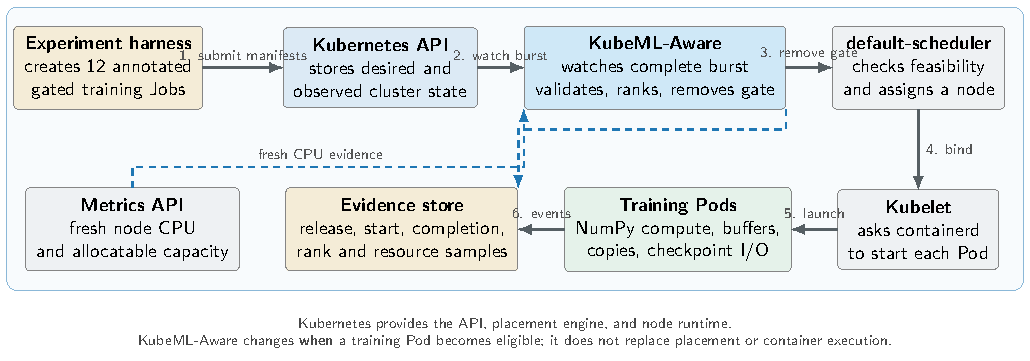
\includegraphics[width=\textwidth]{figures/fig_kubernetes_context.pdf}
  \caption{Kubernetes context and the deployed \system{} control path. Solid arrows show the normal submission-to-execution path. Dashed arrows show telemetry and persistent experiment evidence. The shaded region is the single-node K3s cluster used in the pilot.}
  \label{fig:kubernetes-context}
\end{figure*}

\subsection{Control path and safety boundary}

Fig.~\ref{fig:architecture} summarizes the deployed path. A seeded generator creates a complete burst whose Pods share a run identifier and expected burst size. Each Pod carries six training annotations and the \texttt{ml.scheduler/release} scheduling gate. Resource requests and limits bound demand, and every Pod continues to name \texttt{default-scheduler}.

\begin{figure*}[t]
  \centering
  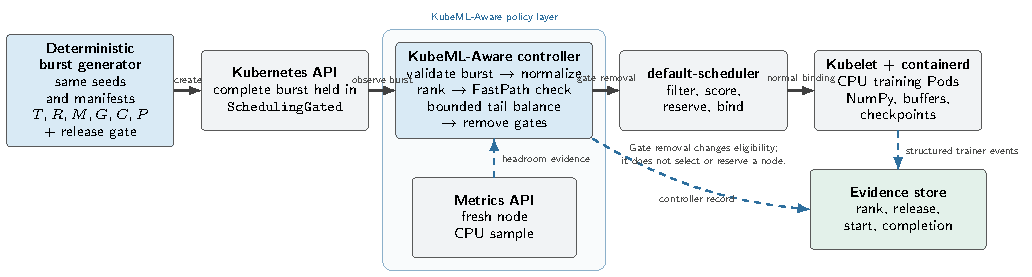
\includegraphics[width=\textwidth]{figures/fig_architecture.pdf}
  \caption{Deployed \system{} architecture. The controller regulates eligibility, not placement. Gate removal hands a Pod to the normal Kubernetes scheduler; structured trainer events and controller records provide an auditable execution trace.}
  \label{fig:architecture}
\end{figure*}

The controller accepts a burst only after exactly the declared number of Pods has appeared and membership has remained unchanged for a short quiet interval. Missing features, duplicate identifiers, inconsistent run metadata, non-finite values, or unexpected external gate changes fail the run rather than silently changing its meaning. Equal scores are resolved using creation time, UID, and name so that Kubernetes API list order cannot affect the result.

Every transition is persisted before the next mutation. The record contains Pod UIDs, feature values, ranks, intended release order, FastPath evidence, release times, and observed execution events. After a restart, the controller relists the burst and reconciles only operations whose UID and state still match. This record is also the basis for result collection.

\subsection{Burst-relative training rank}

For job $j$, the feature vector is $\mathcal{F}=\{T,R,M,G,C,P\}$. In the implemented proxy, $T$ is estimated training time, $R$ controls loss reduction, $M$ is the square-matrix dimension, $G$ is the physical gradient-buffer size, $C$ is the checkpoint interval, and $P$ controls partition and synchronization work. Larger $R$ and $C$ are preferred; smaller $T$, $M$, $G$, and $P$ are preferred. In particular, $P$ is not a GPU count in the present CPU-only system.

Each feature is normalized within its own burst. For feature $k$ of job $j$,
\begin{equation}
\hat{x}_{k,j}=
\begin{cases}
\dfrac{x_{k,j}-x_k^{\min}}{x_k^{\max}-x_k^{\min}}, & k\in\{R,C\},\\[6pt]
\dfrac{x_k^{\max}-x_{k,j}}{x_k^{\max}-x_k^{\min}}, & k\in\{T,M,G,P\}.
\end{cases}
\label{eq:normalization}
\end{equation}
If $x_k^{\max}=x_k^{\min}$, every job receives $\hat{x}_{k,j}=0.5$ for that feature. This makes the term neutral rather than rewarding an arbitrary job.

The base score is
\begin{equation}
S_j=0.32\hat{T}_j+0.28\hat{R}_j+0.16\hat{M}_j+0.12\hat{G}_j+0.08\hat{C}_j+0.04\hat{P}_j.
\label{eq:rank}
\end{equation}
Jobs are sorted by decreasing $S_j$. The coefficients are fixed before evaluation and sum to 1. Scaling all coefficients by the same positive constant would not change the order. In the current generator, $T$ is derived from the other five features, so the terms are not statistically independent. The score should consequently be read as an explicit policy, not a learned predictor or an optimality proof. Scores are also local to one burst and cannot be compared across runs.

\subsection{Training FastPath}

The conservative controller releases the highest-ranked Pod and waits for its application-level start marker before moving to the next job. This protects the intended prefix when startup conditions are uncertain, but it can leave the scheduler queue empty between releases. FastPath addresses that bubble without bypassing Kubernetes capacity checks.

A burst is FastPath-eligible only when it is training-only, uses no experimental pacing or reversed order, every application and initialization container has bounded CPU demand, and a fresh Metrics API sample is available~\cite{kubernetesMetrics}. Let $u$ be measured node CPU utilization, $D$ the sum of declared peak Pod demand, $A$ allocatable CPU, and $\tau=0.85$ the configured threshold. The controller computes
\begin{equation}
u_{\mathrm{projected}}=u+\frac{D}{A}.
\label{eq:headroom}
\end{equation}
If the whole burst fits, all gates are removed in ranked order. If at least one ranked Pod fits but the burst exceeds current headroom, the implementation still prefills the complete ranked queue; the default scheduler then keeps infeasible Pods pending according to their normal requests and constraints. If telemetry is stale or no bounded demand can be established, FastPath fails closed and the controller returns to the conservative path.

Before queue prefill, the controller may permute at most the four lowest-ranked jobs. It predicts a list schedule from $T$, keeps the high-priority prefix fixed, and chooses the suffix with the lowest predicted makespan, using cumulative completion time as a secondary criterion. At most $4! = 24$ permutations are examined. Validation and feature normalization are $O(N)$, ranking is $O(N\log N)$, and the bounded suffix search does not change the asymptotic complexity.

\section{Workload and Experimental Method}

\subsection{Controlled training proxy}

The experiment uses work-model version 2.0 and a containerized NumPy trainer~\cite{harris2020numpy}. For each step, the process multiplies partitions of two $M\times M$ float matrices, updates a $G$-MiB gradient buffer, and performs $P-1$ physical buffer copies when $P>1$. Synthetic loss follows
\begin{equation}
L_{s+1}=L_s e^{-R},
\end{equation}
and training stops at the convergence threshold or a bounded step budget. Every $C$ steps, the process writes a bounded model-state payload and calls \texttt{fsync}. $T$ is estimated from this versioned work model; it does not terminate the process.

The reported pilot uses the heavy profile only: $R\in[0.03,0.08]$, $M\in[512,1024]$, $G\in[20,50]$~MiB, $C\in[20,50]$ steps, and $P\in[2,4]$. BLAS is restricted and attested to one thread. The workload exercises real CPU, memory, copying, and local I/O, but it is not a neural network, does not read a dataset, uses no GPU, and performs no inter-node communication. The shared parameters between the ranker and proxy make the pilot suitable for validating the control path, but not for establishing robustness to feature-estimation error.

\subsection{Cluster and paired protocol}

\system{} was implemented as a Python controller running inside Kubernetes, not as an offline simulator. All measurements reported here were produced by Kubernetes Jobs that reached completion on the deployed cluster and emitted structured execution-start and completion events. Table~\ref{tab:platform} records the platform observed during the experiment.

\begin{table}[t]
\caption{Recorded Experimental Platform}
\label{tab:platform}
\centering
\footnotesize
\begin{tabularx}{\columnwidth}{@{}lX@{}}
\toprule
Component & Recorded configuration \\
\midrule
Virtual machine & KVM; x86-64 architecture \\
Processor & 4 vCPU; Intel Xeon Gold 6138 at 2.00~GHz \\
Memory & 7.57~GiB installed \\
Operating system & Ubuntu 22.04.5 LTS; Linux 5.15.0-177-generic \\
Orchestrator & Single-node K3s/Kubernetes v1.36.2+k3s1; control-plane Ready \\
Container runtime & containerd 2.3.2-k3s2 \\
Training image & \path{registry.local/kubeml/ml-sim-job:0.3.0} \\
Pod resources & 1 vCPU request/limit; 128~MiB request; 1~GiB limit \\
\bottomrule
\end{tabularx}
\end{table}

The operational node also hosted VPN, ingress, monitoring, and Knative-related services. Before each arm, the harness required two CPU samples at or below 35\%, five seconds apart, and verified the protected VPN services. Their readiness and restart counts did not change during the experiment.

Five paired repetitions used seeds 8100--8104. Every repetition generated 12 source jobs, and the baseline and \system{} arms received identical feature values, trainer image, random seeds, resource declarations, and work-model version. The arms ran sequentially in separate namespaces and never overlapped. Arm order alternated: the baseline ran first in repetitions 0, 2, and 4; \system{} ran first in repetitions 1 and 3.

Both arms used the same initial scheduling gate to remove sequential API-submission spread. The baseline removed gates in manifest/FIFO order after the full burst had been observed. The \system{} arm removed the same gates in its ranked, tail-balanced FastPath order. Both arms used \texttt{default-scheduler}; neither manually bound Pods. Thus the comparison isolates admission policy more closely than a baseline whose Pods become eligible as they are created.

For job $j$, $\jct_j=c_j-s_j$, where $s_j$ is Pod creation time and $c_j$ is the application-level completion time. Using Pod creation for $s_j$ deliberately keeps scheduling and queueing latency---the quantity the admission policy affects---inside the measured JCT. Makespan is $\max_j(c_j)-\min_j(s_j)$. The p95 JCT uses linear interpolation over the 12 job values. For metric $m$ in repetition $r$, paired improvement is
\begin{equation}
I_{m,r}=100\frac{m_{\mathrm{FIFO},r}-m_{\system,r}}{m_{\mathrm{FIFO},r}}.
\end{equation}
Positive values mean that \system{} reduced the metric. We report the mean of the five within-pair percentages. Exploratory 95\% intervals use a Student-$t$ interval over those five paired effects; given the small sample and shared host, they are descriptive rather than confirmatory.

\section{Results and Discussion}

\subsection{Paired pilot results}

Table~\ref{tab:results} and Fig.~\ref{fig:results} summarize the five repetitions. Average JCT improved in every pair, with individual reductions from 3.32\% to 12.79\%. The mean paired improvement was 7.31\%, and the exploratory 95\% interval was [2.57\%, 12.05\%]. The corresponding grand means were 31.047~s for FIFO and 28.755~s for \system.

\begin{table}[t]
\caption{Five-Pair Heavy-Training Pilot}
\label{tab:results}
\centering
\footnotesize
\setlength{\tabcolsep}{2.5pt}
\begin{tabular}{lrrrr}
\toprule
Metric & FIFO & \system{} & Paired change & 95\% interval \\
\midrule
Average JCT & 31.047 s & 28.755 s & $+7.31\%$ & [2.57, 12.05] \\
Makespan    & 55.369 s & 54.005 s & $+2.47\%$ & [$-0.45$, 5.40] \\
\bottomrule
\end{tabular}
\end{table}

Makespan also improved in all five pairs, but by a smaller and more variable amount: 0.55\% to 5.87\%, with a mean paired improvement of 2.47\%. Its exploratory interval crosses zero. The consistency of the observed direction is encouraging, but five runs on a shared node do not support a general throughput claim.

As a secondary diagnostic, p95 JCT changed from 52.896 to 53.270~s (a 0.75\% paired regression). With only 12 jobs per arm, this percentile lies close to the maximum and is unstable; it is therefore not used as a headline outcome. The observation nevertheless indicates that a future policy should include an explicit tail-latency or aging objective.

\begin{figure*}[t]
  \centering
  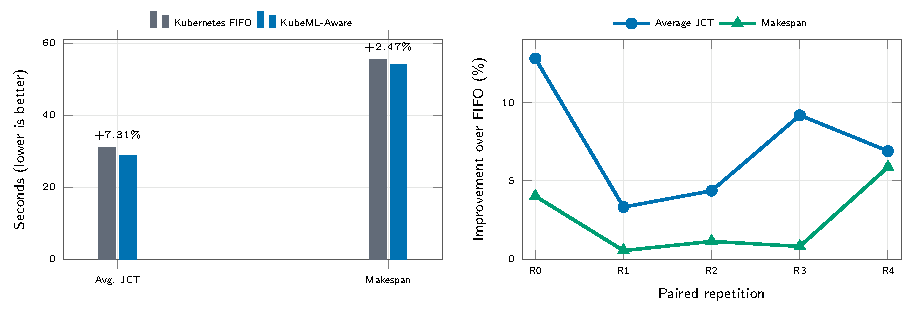
\includegraphics[width=0.98\textwidth]{figures/fig_results.pdf}
  \caption{Primary aggregate and paired pilot results. Bars show five-repetition means. Lines show within-pair improvement, where positive values indicate lower time under \system. Average JCT and makespan improved in all five pairs.}
  \label{fig:results}
\end{figure*}

Fig.~\ref{fig:timeline} visualizes application-level execution intervals for repetition 0. The FIFO arm largely follows manifest order, whereas \system{} brings several jobs from later manifest positions into the first execution wave. This is direct evidence that the gate policy changed admission and observed start order. It is not, by itself, evidence that the six-feature equation, queue prefill, or tail optimizer caused a particular fraction of the final improvement.

\begin{figure*}[t]
  \centering
  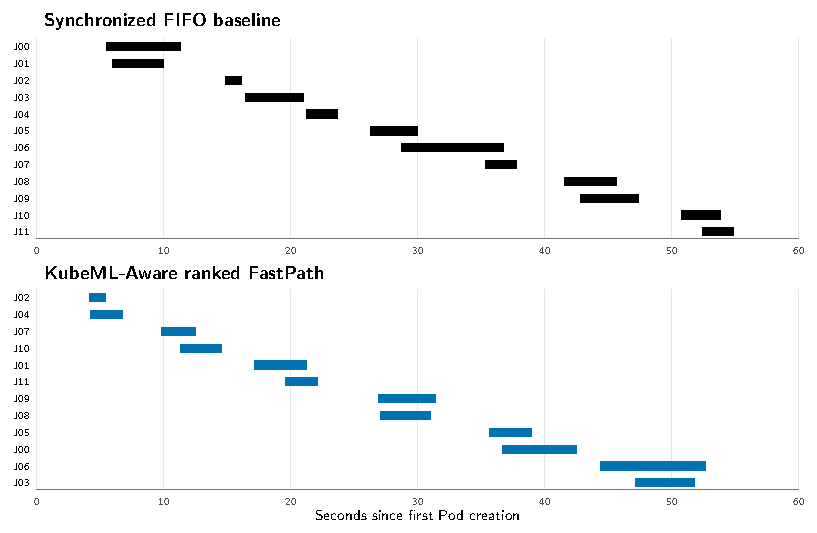
\includegraphics[width=0.81\textwidth]{figures/fig_timeline.pdf}
  \caption{Application-level execution intervals for repetition 0. Labels identify the same source-job indices in both arms; rows are ordered by observed execution start. The reordering is visible, while overlap shows that FastPath preserves concurrency rather than serializing the burst.}
  \label{fig:timeline}
\end{figure*}

\subsection{Threats to validity}

The main threat is the environment. The evaluation node was an operational server, not an isolated benchmark host. Alternating arm order, paired inputs, cool-node checks, and unchanged protected-service state reduce systematic bias, but cannot remove background variation. We therefore label this run as a production-path pilot rather than a isolated benchmark.

Second, the evaluation contains only five pairs and one 12-job heavy profile. The intervals in Table~\ref{tab:results} depend on a small-sample normality assumption and should not be read as definitive significance tests. A tail percentile estimated from 12 observations per arm is especially weak.

Third, the controlled trainer shares its feature semantics with the ranking policy. That choice makes workload behavior auditable and prevents sleep-based simulation, but it may favor a rank whose inputs were designed around the same cost model. Real PyTorch or TensorFlow jobs can exhibit data stalls, framework overhead, GPU kernels, communication, and convergence error that this proxy does not represent.

Finally, the measured treatment combines six-feature ranking, queue prefill, and bounded tail balancing. No live duration-only, reversed-order, FastPath-without-tail, or alternative-weight arm was included. The pilot therefore measures the deployed policy as a whole and cannot assign causality to one component. These limitations are part of the result boundary, not future details that can be assumed away.

\section{Conclusion}

\system{} shows that an ML-specific admission policy can be added to Kubernetes without replacing its placement engine. A controller ranks a complete annotated training burst, removes stable scheduling gates, and uses fresh resource evidence to avoid unnecessary admission gaps. On a shared four-core K3s node, the deployed policy reduced mean JCT by 7.31\% across five paired 12-job runs (exploratory 95\% CI [2.57\%, 12.05\%]); makespan moved in the same direction (2.47\%) but its interval includes zero and is not an established effect. Both metrics decreased in every pair.

The result is promising but preliminary. The next evaluation should run on a dedicated cluster with more repetitions, predeclared ablations, and real framework workloads. GPU and multi-node experiments must give $G$ and $P$ measured communication and parallelism semantics; profiling should replace generator-provided estimates; and aging or an explicit tail objective should improve robustness. Source code and experiment artifacts are available at \url{https://github.com/AmirMirzaeiMovahed/KubeML-Aware}.

\bibliographystyle{IEEEtran}
\bibliography{references}

\end{document}
